\section{Image Formation}
Images are formed when a sensor registers radiation that has interacted with a physical object. e.g. light bouncing off something into your eye

\begin{description}
    \item[Illuminance] Light from source$\rightarrow$ object
    \item[Luminance] Light from object $\rightarrow$ sensor. 
\end{description}
Luminance is a function of the illuminance and the reflectance (Reflective properties) of the object

\subsection{Factors}
The images formed are affected by two sets of parameters:
\begin{enumerate}
    \item Radiometric parameters - these determine the intensity/colour of a section of the image. e.g. illuminance type, object reflectance, sensor properties
    \item Geometric Parameters - where the 3d points is mapped to in the 2d image. e.g. sensor position/orientation, focal length
\end{enumerate}

\subsection{Definitions}
\emph{Light} is electromagnetic waves with wavelength($\lambda$) in the range (400nm,700nm). Human eyes are specialised sensors that are sensitive to this part of the spectrum, and use it for vision. Images can be formed by other waves. e.g infrared cameras, X-ray\\

Human eyes see different wavelengths as different colours - each source of light emits different amounts of each wavelength, which vary the colour we see them as. \emph{Albedo} is the fraction of light a surface reflects at each wavelength - this gives objects their natural colours. e.g. A ripe tomato reflects red (700nm) well, and doesn't reflect blue (400nm). \\

Mixing lights is additive - it gives a white light. Mixing pigments is subtractive - we get a black surface (Albedo of 0 for every colour, as it absorbs everything). \\

Colours aren't a property of the world - the human visual system uses it to represent the albedo of a surface. Determining colour is an ill-posed problem for vision systems, as it depends on illuminance and albedo. Humans are able to naturally determine colours without knowing the exact illuminance.  


\subsection{Focusing Images}
Since light reflects off everything, a sensor would just give us the average illumination. Optics can be used to \emph{focus} light rays onto the sensor to get a useful output.
\begin{description}
    \item[Focus] All rays from a point in the world converge on a single point in the image. This can be done by placing a small aperture between the sensor and the scene (i.e a pinhole camera)
    \item[Exposure] Time required for the sensor to get enough radiation to measure. Too long gives a blurry image, as the luminance tends to average.
\end{description}
\[
Focus \propto \frac{1}{Exposure} \propto \frac{1}{Aperture Size}
\]
A larger pinhole gives a brighter image, but makes it blurrier (more average luminance).

\subsection{Lenses}
A lens can be used to allow in light, while focusing the scene. It specifically focuses a part of the scene at a specific length from the lens (\emph{focal length}), which somewhat limits it. \\
A lens is a thin transparent curved piece (usually glass/plastic) that refracts light. 
\begin{description}
    \item[Optical Centre] Centre of the lens, light rays that pass through this remain unchanged
    \item[Optical Axis] The line passing through the optical centre and perpendicular to the lens. \\ \quad \quad Rays that pass parallel to the optical axis pass through the focal point after refraction.
    \item[Focal Point] The point on the optical axis that represents the focal length of the lens. \\ \quad \quad Rays that pass through the focal length before refraction are parallel to the optical axis after refraction.
\end{description}

In the below image (from the slides): F and F' are the focal points, O is the optical centre, $f$ is the focal length, and the red lines show the three light rays we consider for simple models.  $Z'$ and $z$ are the distance of the object and image from the lens respectively. 
\begin{figure}[H]
    \centering
    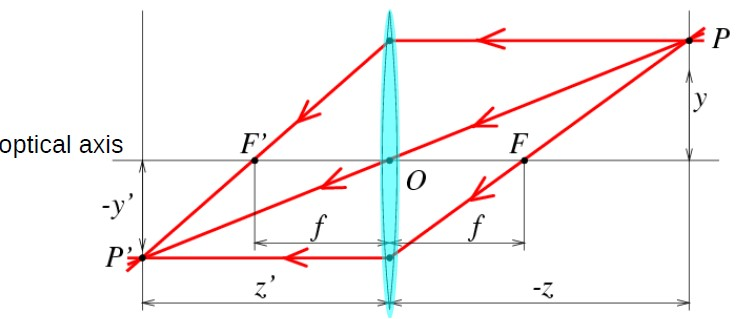
\includegraphics[width = \textwidth]{Images/Thin_Lens_Diagram}
\end{figure}

\subsubsection{Thin Lens Equation}
\begin{equation}
    \frac{1}{f} = \frac{1}{|z|} + \frac{1}{|z'|}
\end{equation}
Where z is the distance between the lens/object, and z' is the distance between lens/image. 

According to the above, objects at infinity will be formed at f - all the scene points will be focused at a single image point, so no meaningful image. For any object closer than f, the light rays won't converge and no image will form. Realistically, anything just beyond 2f and closer will form a meaningful image - the receptor plane is normally placed between (F', 2F'). 

\subsubsection{Focal Range}
The \emph{focal range} is the range that an object can be moved without noticing a blur in the image.\\ The smaller the aperture/lens size, the larger the focal range (but the darker the image, as less light comes in). A pinhole camera has an infinite focal range. 

\subsection{Perspective/Pinhole camera model}\label{subsec:Camera_Model}
A simple camera model that only considers rays passing through the optical centre, and assumes the image plane is at F'. As a pinhole camera, images are always in focus. 
\begin{figure}[H]
    \centering
    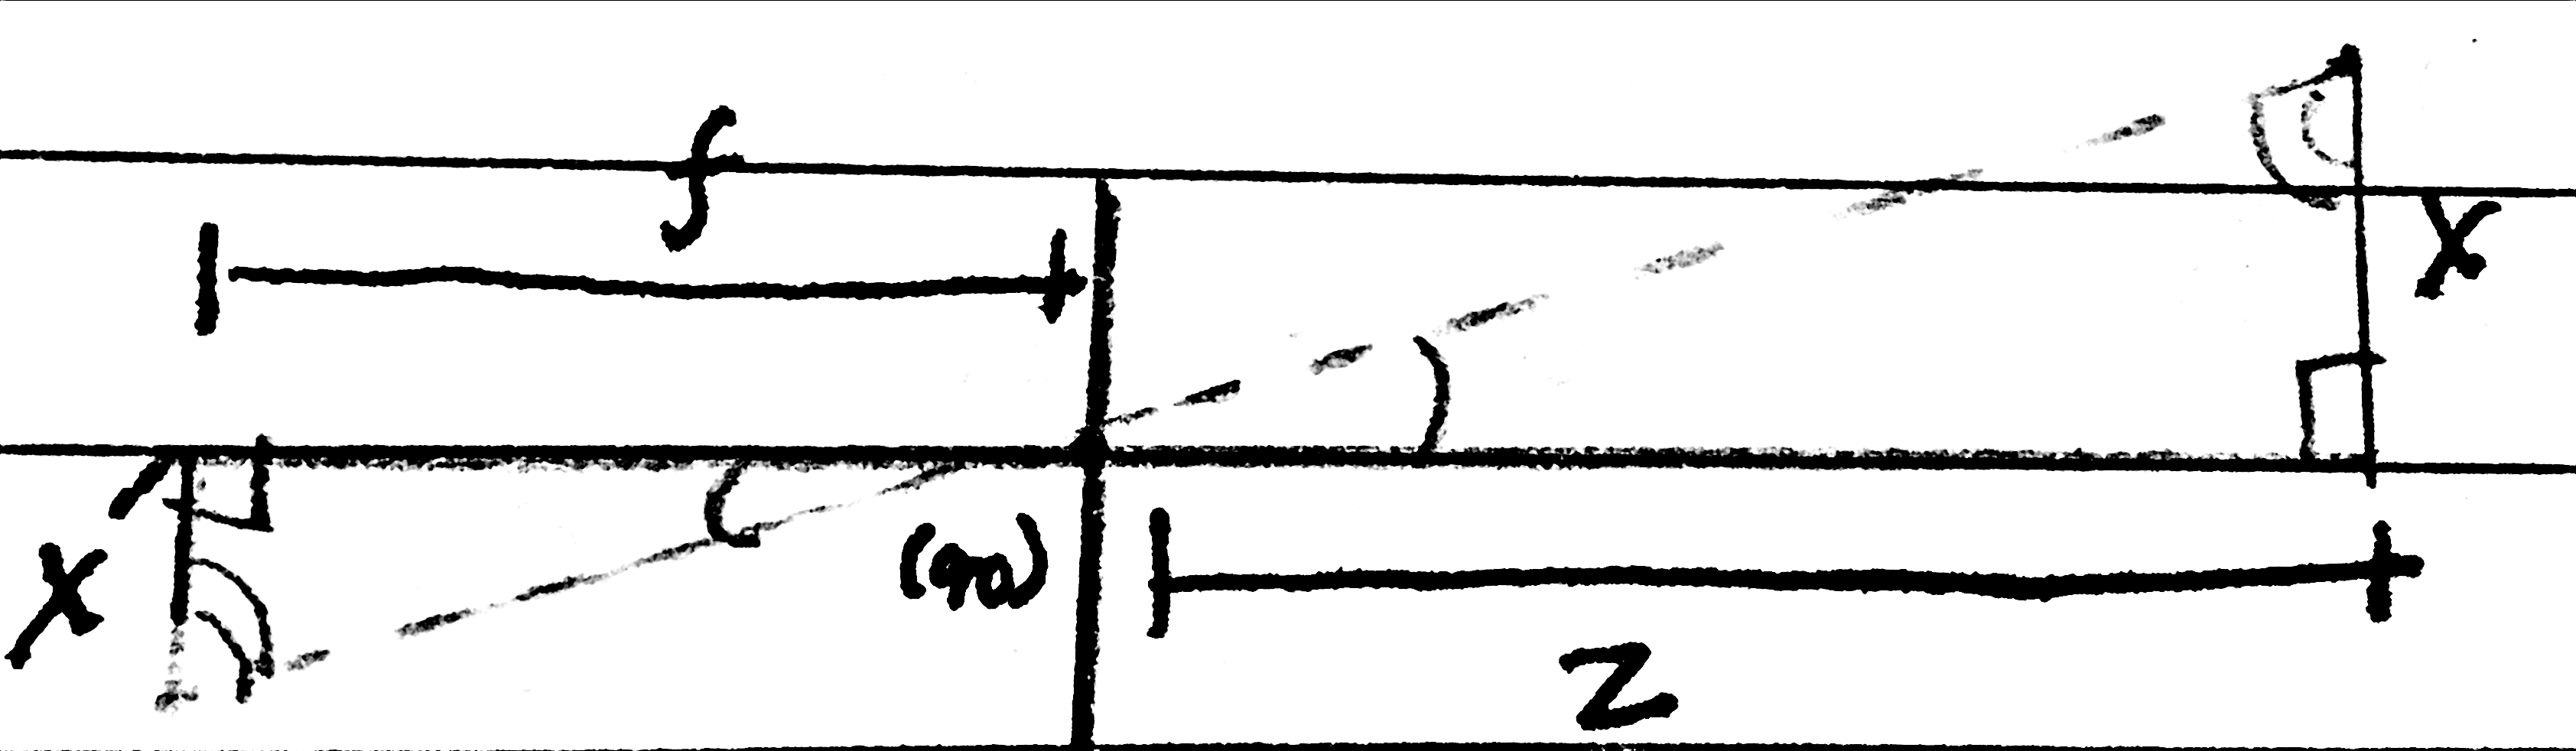
\includegraphics[width = \textwidth]{Images/Pinhole_Model}
\end{figure}
By using similar triangles, we can say that:
\begin{equation}
    X' = \frac{f}{z}\cdot X
\end{equation}
A similar calculation can be done to find the Y co-ordinate of the point, as Z' is fixed at f' (image plane distance).

\subsubsection{3D to 2D transformation}
Applying the above, we obtain the equation:
\begin{align}
      \begin{pmatrix}
    x' \\ y'\\ z'
    \end{pmatrix}
    &= \frac{f'}{z} \cdot 
    \begin{pmatrix}
    1 & 0 & 0 & 0\\ 0 & 1 & 0 & 0\\ 0 & 0 & 1 & 0
    \end{pmatrix}
    \cdot     \begin{pmatrix}
    x \\ y\\ z\\ 1
    \end{pmatrix}  \\
    &= \frac{focalLength}{objectDistance} \cdot
    \text{Projection Operator} \cdot \text{Camera coordinates} \nonumber
\end{align}
The projection operator is determined by the camera model used - for the simple model, it has no effect. The co-ordinates are relative to the camera's optic centre, rather than the image (as seen in the below image from the slides). 
\begin{figure}[H]
    \centering
    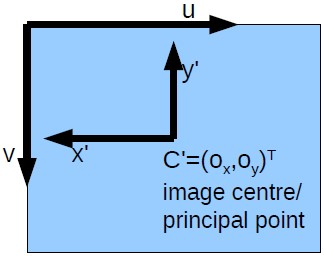
\includegraphics[width = \textwidth, height=7cm,keepaspectratio ]{Images/Coordinate_conversion}
\end{figure}

\subsubsection{Co-ordinate conversion}
To change from camera co-ordinates (mm, (0,0) in centre) to image co-ordinates (px, (0,0) in top left corner), we can use the following equations:
\begin{align}
    u &= \frac{x'}{\frac{mm}{px}} + \text{Optic Centre$_x$} = x \cdot \frac{f'}{z} \cdot \frac{1}{S_x} + O_x = \alpha \cdot \frac{x}{z} + O_x \nonumber \\
    v &= \frac{y'}{\frac{mm}{px}} + \text{Optic Centre$_y$} = y \cdot \frac{f'}{z} \cdot \frac{1}{S_y} + O_x = \beta \cdot \frac{y}{z} + O_x \nonumber     
\end{align}
Where $S_x,S_y$ and $f'$ are constants - $\frac{f'}{S_x} = \alpha$, $\frac{f'}{S_y} = \beta$\\ and $\frac{\alpha}{\beta}$ is the camera's aspect ratio. 
Fitting this into our previous equation, we get:
\begin{align}
      \begin{pmatrix}
    u \\ v \\ 1
    \end{pmatrix}
    &=  \frac{1}{z} \cdot 
    \begin{pmatrix}
    \alpha & 0 & O_x\\
    0 & \beta & O_y \\
    0 & 0 & 1 
    \end{pmatrix} \cdot 
    \begin{pmatrix}
    1 & 0 & 0 & 0\\
    0 & 1 & 0 & 0\\
    0 & 0 & 1 & 0
    \end{pmatrix}
    \cdot     \begin{pmatrix}
    x \\ y\\ z\\ 1
    \end{pmatrix}  \\
    &= \text{Camera parameters} \cdot
    \text{Projection Operator} \cdot \text{Camera coordinates} \nonumber
\end{align}

\subsubsection{Scene Co-ordinates}
Camera co-ordinates are fine, but it's more useful to have an external fixed reference (scene co-ordinates). To convert, we use the camera's inverse translation and rotation matrices:
\begin{equation}
    \begin{pmatrix}
    x \\ y\\ z\\1
    \end{pmatrix}
    =  
    \begin{pmatrix}
    R & t \\
    O^T_3 & 1
    \end{pmatrix}
    \cdot     \begin{pmatrix}
    X \\ Y\\ Z\\1
    \end{pmatrix}
\end{equation}
Where R is a 3 by 3 rotation matrix, t is a 3 by 1 translation matrix, $O_3$ is a 3 by 3 zeroes matrix, and 1 is a single element. After applying the inverse and combining this with the previous equation, we get the complete transformation as:
\begin{align}
      \begin{pmatrix}
    u \\ v \\ 1
    \end{pmatrix}
    &=  \frac{1}{z} \cdot
    \begin{pmatrix}
    \alpha & 0 & O_x\\
    0 & \beta & O_y \\
    0 & 0 & 1 
    \end{pmatrix} \cdot 
    \begin{pmatrix}
    1 & 0 & 0 & 0\\
    0 & 1 & 0 & 0\\
    0 & 0 & 1 & 0
    \end{pmatrix}
    \cdot   
    \begin{pmatrix}
    R^T & -R^Tt \\
    O^T_3 & 1
    \end{pmatrix}
    \cdot
    \begin{pmatrix}
    X \\ Y\\ Z\\ 1
    \end{pmatrix}  \\
    &= \text{Internal camera parameters}(2D \rightarrow 2D)  \cdot
    \text{Projection Operator}(3D\rightarrow 2D) \cdot \nonumber \\ &\quad \quad \text{External camera parameters}(3D\rightarrow 3D) \cdot  \text{World coordinates} \nonumber
\end{align}

\subsubsection{Results}
The above gives us a well-defined equation from 3D to 2D. However, since we're not given Z when doing 2D to 3D, that's an ill-posed problem. \\

For convenience, we use a \emph{Virtual Image} - this is the right side up on the same size as the object, otherwise the same as the actual image. 

\subsection{Projective Geometry}
\begin{description}
    \item[Euclidean Geometry] Translations/transformations in a 3D world
    \item[Projective Geometry] Converts from the 3D to the 2D world (translation, transformation, shear, scaling).
\end{description}
Projective doesn't preserve the shape or angle of the objects, and the size depends on the object distance.

\subsubsection{Vanishing Point}
The \emph{vanishing point} is the projection of the point at infinity in the image. e.g. a long line away from the camera slowly appears to bend towards the focal point in the image\\

Parallel lines have the same vanishing point. e.g. looking along train tracks. The human visual system uses this to determine sizes (e.g. two similar objects along a vanishing parallel line, even though the more distant one appears smaller we think they're the same size)

\subsection{Digital Image Representation}
Digital images have discrete samples of a continuous image (Pixelisation)- each sample is called a picture element (pixel). Each pixel is the average of the intensity value around each sampling point .

These average values are represented with discrete values (Quantization).The more values, the more detailed the picture:
\begin{description}
    \item[Binary Images] Each pixel is 0 or 1
    \item[Greyscale] Each pixel is a single real value (usually 8bit, which has 256 intensities). \\ \quad\quad  - To convert to a binary image, use a threshold function.
    \item[Colour RGB] Each pixel has 3  real values - one for Red, Green and Blue intensities respectively (usually 24 bits in total per pixel). \\ \quad\quad  - To convert to a greyscale image, take the average of the intensities.    
\end{description}

\subsection{Charge Coupled Device Camera}
A sensor consisting of a semiconductor with a 2D matrix of photo-sensors. The more light incident on the camera, the more charge flows through the conductor ($\propto$ intensity, exposure time). Micro-lenses are fit on top of each sensor to better focus the light.\\

For colour, we can use a prism to split the incoming light into colours and measure with 3 separate CCD devices (for R, G and B). Alternatively (and more efficiently), we can use a chequered filter over the whole device, so each photo-sensor only accepts a specific colour. A common filter is the \emph{Bayer Mask}, which has twice as many green as red or blue (since humans are most sensitive to green). \\

As each sensor only accepts one colour, the missing values have to be filled in via \emph{Demosaicing}, which uses interpolation. Some demosaicing methods are: 
\begin{enumerate}
    \item Nearest Neighbour - Copy the closest pixel of the required colour. Fast and inaccurate
    \item Bilinear - Take the average of nearby pixels of the required colour. Fast, not so accurate at edges (since less neighbouring pixels)
    \item Smooth Hue Transition
    \item Edge Directed Interpolation
\end{enumerate}

\subsubsection{Smooth Hue Transition}
Uses information from neighbouring pixels, rather than the raw values:
\begin{description}
    \item[Green] Just take the average of the raw values of neighbours
    \item[Red/Blue] \begin{equation}
        \text{Green value of pixel} \cdot \frac{(\frac{\text(Red/Blue Value)}{(Green Value)}) \text{for each neighbouring pixel}}{\text{Number of neighbouring Red/Blue pixels}} 
    \end{equation}
    i.e. Green Value x Bilinear interpolation of ratio (Hue) between Red/Blue and Green
\end{description}

\subsubsection{Edge-Directed Interpolation}
Just taking an average (As in bilinear and smooth hue) will blur edges, so have an additional check to not interpolate across edges (i.e. interpolate where change in value is lowest) 
\begin{description}
    \item[Green] For a pixel (x,y): 
    \begin{itemize}
        \item $\Delta H = |G(x-1,y) - G(x+1,y)|$, $\Delta V = |G(x,y-1) - G(x,y+1)|$
        \item If $\Delta H < \Delta V$: $G(x,y) =\frac{ G(x-1,y) + G(x+1,y)}{2}$
        \item If $\Delta H > \Delta V$: $G(x,y) =\frac{ G(x,y-1) + G(x,y+1)}{2}$
        \item If $\Delta H = \Delta V$: $G(x,y) =\frac{ G(x-1,y) + G(x+1,y) + G(x,y-1) + G(x,y+1)}{4}$        
    \end{itemize}
    \item[Red/Blue] Same as Smooth Hue transition
\end{description}

\subsection{Image Formation in Humans}
The human eye consists of:
\begin{description}
    \item[Cornea] The first lens, which has a fixed focal length
    \item[Lens] The second lens, which can be stretched to adjust the focal length
    \item[Iris] The aperture, which can adjust to allow more light/better focus
    \item[Retina] The image plane, which contains millions of photoreceptors that transduce light to electricity. 
    \begin{description}
        \item [Fovea] The centre of the image, with the best clarity
        \item[Blind Spot] Where the optic nerve connects to the retina, no vision here
    \end{description}
\end{description}

\subsubsection{Retina}
The retina consists of layers of transparent cells, with the photoreceptors at the back. There are two types of photoreceptors:
\begin{description}
    \item[Rods] High sensitivity, so can work in low light
    \item[Cones] Lower sensitivity so need bright light, but there are three subtypes that are sensitive to R, G and B wavelengths respectively
\end{description}
The retina has more cones in the fovea (blue $<<$ red, $<=$ green), and more rods at the edges (and overall). The fovea has higher resolution, so more processing space in the brain is allocated to it. 

\subsubsection{Gangilon cells}
Gangilon cells collect the information from photoreceptors: near the edges of the eye, 100s of photoreceptors can connect to a single gangilon, leading to lower resolution than the centre. The cells connect and combine to become the optic nerve, and transmit binary signals.\\

The \emph{Receptive Field} of the gangilon is the area of the retina that the cell receives information from: roughly circular. This is usually split into a circular centre and a surrounding ring. \\

Gangilons are either on-centre/off-surround or off-centre/on-surround. These send output when the centre/surround is excited, and inhibit when the surround/centre is excited respectively. 
\begin{description}
    \item [On is excited, Off isn't] Outputs more 1s
    \item[Off is excited, On isn't] Outputs more 0s
    \item[Both/Neither are excited] Outputs a stream of 50/50 1s and 0s
\end{description}
This structure gives better edge detection, as the only 'different' signals are those where an edge has been detected. This doesn't take into account the illumination, only the contrast. As only the cells for strong contrast areas are active, this allows for more efficient encoding as well - less neurons are active. The split between the types is roughly 50/50. \\

Ganglion cells can be replicated using Difference of Gaussian filters.

\subsubsection{Colour Detection}
Colour-Opponent gangilon cells look for blending or opposition between fixed pairs of colours (R/G,B/Yellow) and each pair having on/off centre/surround variants. e.g. on-red-centre/off-green-surround, off-blue-centre/on-yellow-surround \\

They then trigger when certain colours have been found. e.g. Some cells will trigger on Red or Green, but none will trigger for a red/green hybrid